\documentclass [a4paper, 12x `pt]{article}
\usepackage [utf8] {inputenc}
\usepackage [T2A] {fontenc}
\usepackage [russian] {babel}
\usepackage {amsmath, amsfonts, amssymb, amsthm}
\usepackage{graphicx}

\author{Александров Олег}

\begin{document}

\begin{titlepage}
   \begin{center}
        \hfill \break
        \footnotesize{ФЕДЕРАЛЬНОЕ ГОСУДАРСТВЕННОЕ БЮДЖЕТНОЕ ОБРАЗОВАТЕЛЬНОЕ УЧРЕЖДЕНИЕ}\\ 
        \footnotesize{ВЫСШЕГО ПРОФЕССИОНАЛЬНОГО ОБРАЗОВАНИЯ}\\
        \small{\textbf{«МОСКОВСКИЙ ФИЗКУЛЬТУРНЫЙ ТЕХНИКУМ С УГЛУБЛЕННЫМ ИЗУЧЕНИЕМ ИННОСТРАННЫХ ЯЗЫКОВ»} }\\
        \hfill \break
        \hfill \break
        \hfill \break
        \normalsize{«Физкек-школа прикольных мемов и инфоцыганства»}\\
        \hfill \break
        \hfill \break
        \hfill \break
        \normalsize{Кафедра? Я её не выбрал ещё...}\\
        \hfill\break
        \hfill \break
        \hfill \break
        \hfill \break
        \LARGE{«Начало математического безумия!!!»}\\
        \hfill \break
        \hfill \break
        \hfill \break
        \hfill \break
        \hfill \break
        \hfill \break
        \hfill \break
        \hfill \break
        \hfill \break
        \hfill \break
        \begin{center}
            \normalsize{Работу выполнил}
        \end{center}
        \begin{center}
            \normalsize{Александров Олег Алексеевич}
        \end{center}
        \hfill \break
        \normalsize{Долгопрудный 2023} 
    \end{center}
    \thispagestyle{empty}
\end{titlepage}

Дано f(x) = $$ \cos(5 \cdot x + 7) ^{3}  + \sin(x^{7}  + 8)  $$
Методом пристального взгляда заметим, что!
$$ \cos(5 \cdot x + 7) ^{3}  + \sin(x^{7}  + 8)  $$
\begin{figure}[h]
	\centering
	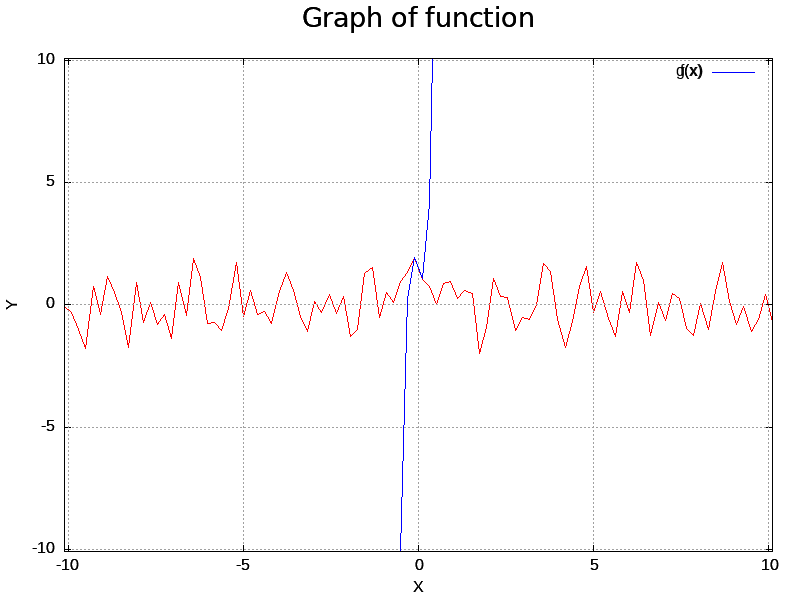
\includegraphics[width=0.8\linewidth]{Images/graphic0.png}
	\caption{\label xGraph of function.}
\end{figure}
"ДИРИХЛЕЕЕЕ!!! ДИРИХЛЕЕЕ!!!" - Савватеев А.В.
$$ \frac{d}{dx}(8) = 0 $$\
Наносим 10 Сталинских ударов по этому выражению!!!
$$ \frac{d}{dx}(x) = 1 $$\
Вспоминаем метод Алекса Эдуардовича Султанова!!!
$$ \frac{d}{dx}(x^{7} ) = 7 \cdot x^{7 - 1}  \cdot 1 $$\
Что это такое? А! Так это очевидно!!!
$$ \frac{d}{dx}(x^{7}  + 8) = 7 \cdot x^{7 - 1}  \cdot 1 + 0 $$\
Получим вот такое выражение! Мы упустили часть доказательств равносильных переходов! Поэтому я хочу, чтобы ВЫ САМИ ИХ ДОКАЗАЛИ!
$$ \frac{d}{dx}(\sin(x^{7}  + 8) ) = \cos(x^{7}  + 8)  \cdot \left(7 \cdot x^{7 - 1}  \cdot 1 + 0\right) $$\
Заметим, что ...
$$ \frac{d}{dx}(7) = 0 $$\
Сейчас наступит катарсис!!!
$$ \frac{d}{dx}(x) = 1 $$\
Наносим 10 Сталинских ударов по этому выражению!!!
$$ \frac{d}{dx}(5) = 0 $$\
Вас ещё не кокнуло? Продолжаем!
$$ \frac{d}{dx}(5 \cdot x) = 0 \cdot x + 5 \cdot 1 $$\
Заметим, что ...
$$ \frac{d}{dx}(5 \cdot x + 7) = 0 \cdot x + 5 \cdot 1 + 0 $$\
Для решения этой задачи переместимся в n-мерное пр-во!!!
$$ \frac{d}{dx}(\cos(5 \cdot x + 7) ) = -1 \cdot \sin(5 \cdot x + 7)  \cdot \left(0 \cdot x + 5 \cdot 1 + 0\right) $$\
Доказательство тривиально!!! Оставим читателю в качестве домашнего упражнения!
$$ \frac{d}{dx}(\cos(5 \cdot x + 7) ^{3} ) = 3 \cdot \cos(5 \cdot x + 7) ^{3 - 1}  \cdot -1 \cdot \sin(5 \cdot x + 7)  \cdot \left(0 \cdot x + 5 \cdot 1 + 0\right) $$\
Для решения этой задачи переместимся в n-мерное пр-во!!!
$$ \frac{d}{dx}(\cos(5 \cdot x + 7) ^{3}  + \sin(x^{7}  + 8) ) = 3 \cdot \cos(5 \cdot x + 7) ^{3 - 1}  \cdot -1 \cdot \sin(5 \cdot x + 7)  \cdot \left(0 \cdot x + 5 \cdot 1 + 0\right) + \cos(x^{7}  + 8)  \cdot \left(7 \cdot x^{7 - 1}  \cdot 1 + 0\right) $$\
Вспоминаем метод Алекса Эдуардовича Султанова!!!
$$ 3 \cdot \cos(5 \cdot x + 7) ^{2}  \cdot -1 \cdot \sin(5 \cdot x + 7)  \cdot 5 + \cos(x^{7}  + 8)  \cdot 7 \cdot x^{6}  $$
В итоге производная f'(x) = $$ 3 \cdot \cos(5 \cdot x + 7) ^{2}  \cdot -1 \cdot \sin(5 \cdot x + 7)  \cdot 5 + \cos(x^{7}  + 8)  \cdot 7 \cdot x^{6}  $$
\begin{figure}[h]
	\centering
	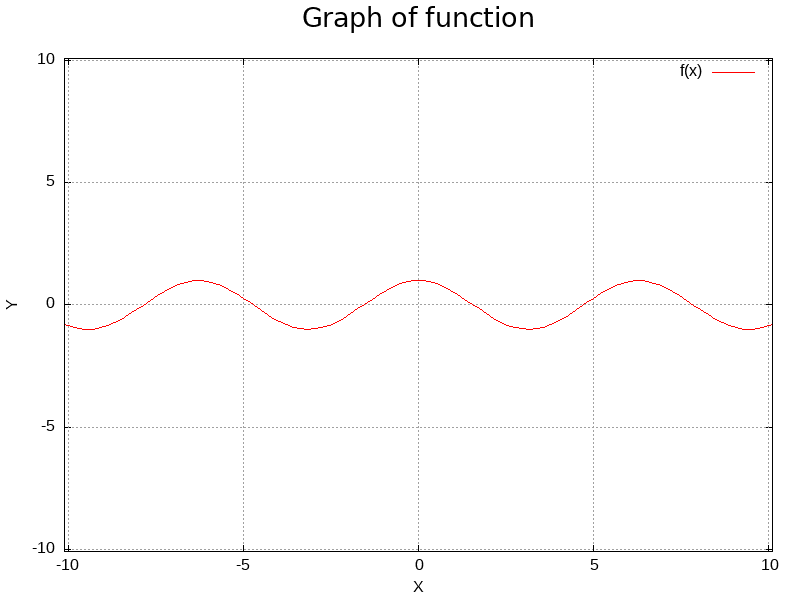
\includegraphics[width=0.8\linewidth]{Images/graphic1.png}
	\caption{\label xGraph of function.}
\end{figure}
"ДИРИХЛЕЕЕЕ!!! ДИРИХЛЕЕЕ!!!" - Савватеев А.В.
$$ \frac{d}{dx}(8) = 0 $$\
Сейчас наступит катарсис!!!
$$ \frac{d}{dx}(x) = 1 $$\
Доказательство тривиально!!! Оставим читателю в качестве домашнего упражнения!
$$ \frac{d}{dx}(x^{7} ) = 7 \cdot x^{7 - 1}  \cdot 1 $$\
"Мне вообще на эти все множители наплевать, делаем. Шлёп, шлёп, шлёп-шлёп!!!" - Райгородский А.М.
$$ \frac{d}{dx}(x^{7}  + 8) = 7 \cdot x^{7 - 1}  \cdot 1 + 0 $$\
Такую задачку решали ещё в советских яслях... Помню, в 1953 году решал её!
$$ \frac{d}{dx}(\sin(x^{7}  + 8) ) = \cos(x^{7}  + 8)  \cdot \left(7 \cdot x^{7 - 1}  \cdot 1 + 0\right) $$\
Для решения этой задачи переместимся в n-мерное пр-во!!!
$$ \frac{d}{dx}(7) = 0 $$\
Такую задачку решали ещё в советских яслях... Помню, в 1953 году решал её!
$$ \frac{d}{dx}(x) = 1 $$\
Методом пристального взгляда заметим, что!
$$ \frac{d}{dx}(5) = 0 $$\
Вас ещё не кокнуло? Продолжаем!
$$ \frac{d}{dx}(5 \cdot x) = 0 \cdot x + 5 \cdot 1 $$\
"ДИРИХЛЕЕЕЕ!!! ДИРИХЛЕЕЕ!!!" - Савватеев А.В.
$$ \frac{d}{dx}(5 \cdot x + 7) = 0 \cdot x + 5 \cdot 1 + 0 $$\
Заметим, что ...
$$ \frac{d}{dx}(\cos(5 \cdot x + 7) ) = -1 \cdot \sin(5 \cdot x + 7)  \cdot \left(0 \cdot x + 5 \cdot 1 + 0\right) $$\
Ну даже ёжику понятно, как посчитать эту производную!!!
$$ \frac{d}{dx}(\cos(5 \cdot x + 7) ^{3} ) = 3 \cdot \cos(5 \cdot x + 7) ^{3 - 1}  \cdot -1 \cdot \sin(5 \cdot x + 7)  \cdot \left(0 \cdot x + 5 \cdot 1 + 0\right) $$\
Вспоминаем метод Алекса Эдуардовича Султанова!!!
$$ \frac{d}{dx}(\cos(5 \cdot x + 7) ^{3}  + \sin(x^{7}  + 8) ) = 3 \cdot \cos(5 \cdot x + 7) ^{3 - 1}  \cdot -1 \cdot \sin(5 \cdot x + 7)  \cdot \left(0 \cdot x + 5 \cdot 1 + 0\right) + \cos(x^{7}  + 8)  \cdot \left(7 \cdot x^{7 - 1}  \cdot 1 + 0\right) $$\
Вспоминаем метод Алекса Эдуардовича Султанова!!!
$$ 3 \cdot \cos(5 \cdot x + 7) ^{2}  \cdot -1 \cdot \sin(5 \cdot x + 7)  \cdot 5 + \cos(x^{7}  + 8)  \cdot 7 \cdot x^{6}  $$
Получим вот такое выражение! Мы упустили часть доказательств равносильных переходов! Поэтому я хочу, чтобы ВЫ САМИ ИХ ДОКАЗАЛИ!
$$ 1.41785 + -5.60116 \cdot x $$
Наносим 10 Сталинских ударов по этому выражению!!!
$$ \frac{d}{dx}(x) = 1 $$\
Заметим, что ...
$$ \frac{d}{dx}(x^{6} ) = 6 \cdot x^{6 - 1}  \cdot 1 $$\
"ДИРИХЛЕЕЕЕ!!! ДИРИХЛЕЕЕ!!!" - Савватеев А.В.
$$ \frac{d}{dx}(7) = 0 $$\
Доказательство тривиально!!! Оставим читателю в качестве домашнего упражнения!
$$ \frac{d}{dx}(7 \cdot x^{6} ) = 0 \cdot x^{6}  + 7 \cdot 6 \cdot x^{6 - 1}  \cdot 1 $$\
Вас ещё не кокнуло? Продолжаем!
$$ \frac{d}{dx}(8) = 0 $$\
Методом пристального взгляда заметим, что!
$$ \frac{d}{dx}(x) = 1 $$\
Что это такое? А! Так это очевидно!!!
$$ \frac{d}{dx}(x^{7} ) = 7 \cdot x^{7 - 1}  \cdot 1 $$\
Такую задачку решали ещё в советских яслях... Помню, в 1953 году решал её!
$$ \frac{d}{dx}(x^{7}  + 8) = 7 \cdot x^{7 - 1}  \cdot 1 + 0 $$\
Вспоминаем метод Алекса Эдуардовича Султанова!!!
$$ \frac{d}{dx}(\cos(x^{7}  + 8) ) = -1 \cdot \sin(x^{7}  + 8)  \cdot \left(7 \cdot x^{7 - 1}  \cdot 1 + 0\right) $$\
Заметим, что ...
$$ \frac{d}{dx}(\cos(x^{7}  + 8)  \cdot 7 \cdot x^{6} ) = -1 \cdot \sin(x^{7}  + 8)  \cdot \left(7 \cdot x^{7 - 1}  \cdot 1 + 0\right) \cdot 7 \cdot x^{6}  + \cos(x^{7}  + 8)  \cdot \left(0 \cdot x^{6}  + 7 \cdot 6 \cdot x^{6 - 1}  \cdot 1\right) $$\
По миллионной теореме Коши для всех случаев в жизни!
$$ \frac{d}{dx}(5) = 0 $$\
Вас ещё не кокнуло? Продолжаем!
$$ \frac{d}{dx}(7) = 0 $$\
По миллионной теореме Коши для всех случаев в жизни!
$$ \frac{d}{dx}(x) = 1 $$\
Методом пристального взгляда заметим, что!
$$ \frac{d}{dx}(5) = 0 $$\
Такую задачку решали ещё в советских яслях... Помню, в 1953 году решал её!
$$ \frac{d}{dx}(5 \cdot x) = 0 \cdot x + 5 \cdot 1 $$\
Наносим 10 Сталинских ударов по этому выражению!!!
$$ \frac{d}{dx}(5 \cdot x + 7) = 0 \cdot x + 5 \cdot 1 + 0 $$\
Ну даже ёжику понятно, как посчитать эту производную!!!
$$ \frac{d}{dx}(\sin(5 \cdot x + 7) ) = \cos(5 \cdot x + 7)  \cdot \left(0 \cdot x + 5 \cdot 1 + 0\right) $$\
"Мне вообще на эти все множители наплевать, делаем. Шлёп, шлёп, шлёп-шлёп!!!" - Райгородский А.М.
$$ \frac{d}{dx}(\sin(5 \cdot x + 7)  \cdot 5) = \cos(5 \cdot x + 7)  \cdot \left(0 \cdot x + 5 \cdot 1 + 0\right) \cdot 5 + \sin(5 \cdot x + 7)  \cdot 0 $$\
Для решения этой задачи переместимся в n-мерное пр-во!!!
$$ \frac{d}{dx}(-1) = 0 $$\
Доказательство тривиально!!! Оставим читателю в качестве домашнего упражнения!
$$ \frac{d}{dx}(-1 \cdot \sin(5 \cdot x + 7)  \cdot 5) = 0 \cdot \sin(5 \cdot x + 7)  \cdot 5 + -1 \cdot \left(\cos(5 \cdot x + 7)  \cdot \left(0 \cdot x + 5 \cdot 1 + 0\right) \cdot 5 + \sin(5 \cdot x + 7)  \cdot 0\right) $$\
Вас ещё не кокнуло? Продолжаем!
$$ \frac{d}{dx}(7) = 0 $$\
"ДИРИХЛЕЕЕЕ!!! ДИРИХЛЕЕЕ!!!" - Савватеев А.В.
$$ \frac{d}{dx}(x) = 1 $$\
Для решения этой задачи переместимся в n-мерное пр-во!!!
$$ \frac{d}{dx}(5) = 0 $$\
"Мне вообще на эти все множители наплевать, делаем. Шлёп, шлёп, шлёп-шлёп!!!" - Райгородский А.М.
$$ \frac{d}{dx}(5 \cdot x) = 0 \cdot x + 5 \cdot 1 $$\
"Мне вообще на эти все множители наплевать, делаем. Шлёп, шлёп, шлёп-шлёп!!!" - Райгородский А.М.
$$ \frac{d}{dx}(5 \cdot x + 7) = 0 \cdot x + 5 \cdot 1 + 0 $$\
Что это такое? А! Так это очевидно!!!
$$ \frac{d}{dx}(\cos(5 \cdot x + 7) ) = -1 \cdot \sin(5 \cdot x + 7)  \cdot \left(0 \cdot x + 5 \cdot 1 + 0\right) $$\
Ну даже ёжику понятно, как посчитать эту производную!!!
$$ \frac{d}{dx}(\cos(5 \cdot x + 7) ^{2} ) = 2 \cdot \cos(5 \cdot x + 7) ^{2 - 1}  \cdot -1 \cdot \sin(5 \cdot x + 7)  \cdot \left(0 \cdot x + 5 \cdot 1 + 0\right) $$\
Доказательство тривиально!!! Оставим читателю в качестве домашнего упражнения!
$$ \frac{d}{dx}(3) = 0 $$\
"Мне вообще на эти все множители наплевать, делаем. Шлёп, шлёп, шлёп-шлёп!!!" - Райгородский А.М.
$$ \frac{d}{dx}(3 \cdot \cos(5 \cdot x + 7) ^{2} ) = 0 \cdot \cos(5 \cdot x + 7) ^{2}  + 3 \cdot 2 \cdot \cos(5 \cdot x + 7) ^{2 - 1}  \cdot -1 \cdot \sin(5 \cdot x + 7)  \cdot \left(0 \cdot x + 5 \cdot 1 + 0\right) $$\
Что это такое? А! Так это очевидно!!!
$$ \frac{d}{dx}(3 \cdot \cos(5 \cdot x + 7) ^{2}  \cdot -1 \cdot \sin(5 \cdot x + 7)  \cdot 5) = \left(0 \cdot \cos(5 \cdot x + 7) ^{2}  + 3 \cdot 2 \cdot \cos(5 \cdot x + 7) ^{2 - 1}  \cdot -1 \cdot \sin(5 \cdot x + 7)  \cdot \left(0 \cdot x + 5 \cdot 1 + 0\right)\right) \cdot -1 \cdot \sin(5 \cdot x + 7)  \cdot 5 + 3 \cdot \cos(5 \cdot x + 7) ^{2}  \cdot \left(0 \cdot \sin(5 \cdot x + 7)  \cdot 5 + -1 \cdot \left(\cos(5 \cdot x + 7)  \cdot \left(0 \cdot x + 5 \cdot 1 + 0\right) \cdot 5 + \sin(5 \cdot x + 7)  \cdot 0\right)\right) $$\
Что это такое? А! Так это очевидно!!!
$$ \frac{d}{dx}(3 \cdot \cos(5 \cdot x + 7) ^{2}  \cdot -1 \cdot \sin(5 \cdot x + 7)  \cdot 5 + \cos(x^{7}  + 8)  \cdot 7 \cdot x^{6} ) = \left(0 \cdot \cos(5 \cdot x + 7) ^{2}  + 3 \cdot 2 \cdot \cos(5 \cdot x + 7) ^{2 - 1}  \cdot -1 \cdot \sin(5 \cdot x + 7)  \cdot \left(0 \cdot x + 5 \cdot 1 + 0\right)\right) \cdot -1 \cdot \sin(5 \cdot x + 7)  \cdot 5 + 3 \cdot \cos(5 \cdot x + 7) ^{2}  \cdot \left(0 \cdot \sin(5 \cdot x + 7)  \cdot 5 + -1 \cdot \left(\cos(5 \cdot x + 7)  \cdot \left(0 \cdot x + 5 \cdot 1 + 0\right) \cdot 5 + \sin(5 \cdot x + 7)  \cdot 0\right)\right) + -1 \cdot \sin(x^{7}  + 8)  \cdot \left(7 \cdot x^{7 - 1}  \cdot 1 + 0\right) \cdot 7 \cdot x^{6}  + \cos(x^{7}  + 8)  \cdot \left(0 \cdot x^{6}  + 7 \cdot 6 \cdot x^{6 - 1}  \cdot 1\right) $$\
Вас ещё не кокнуло? Продолжаем!
$$ 3 \cdot 2 \cdot \cos(5 \cdot x + 7)  \cdot -1 \cdot \sin(5 \cdot x + 7)  \cdot 5 \cdot -1 \cdot \sin(5 \cdot x + 7)  \cdot 5 + 3 \cdot \cos(5 \cdot x + 7) ^{2}  \cdot -1 \cdot \cos(5 \cdot x + 7)  \cdot 5 \cdot 5 + -1 \cdot \sin(x^{7}  + 8)  \cdot 7 \cdot x^{6}  \cdot 7 \cdot x^{6}  + \cos(x^{7}  + 8)  \cdot 7 \cdot 6 \cdot x^{5}  $$
Сейчас наступит катарсис!!!
$$ 1.41785 + -5.60116 \cdot x + 8.33705 \cdot x^{2}  $$
Методом пристального взгляда заметим, что!
$$ \frac{d}{dx}(x) = 1 $$\
"АААаааАААА!!! n-ая Теорема Кантора! Вы не шокированы?? Вы точно поняли?" - Дашков Е.В.
$$ \frac{d}{dx}(x^{5} ) = 5 \cdot x^{5 - 1}  \cdot 1 $$\
Наносим 10 Сталинских ударов по этому выражению!!!
$$ \frac{d}{dx}(6) = 0 $$\
Ну даже ёжику понятно, как посчитать эту производную!!!
$$ \frac{d}{dx}(6 \cdot x^{5} ) = 0 \cdot x^{5}  + 6 \cdot 5 \cdot x^{5 - 1}  \cdot 1 $$\
Что это такое? А! Так это очевидно!!!
$$ \frac{d}{dx}(7) = 0 $$\
Что это такое? А! Так это очевидно!!!
$$ \frac{d}{dx}(7 \cdot 6 \cdot x^{5} ) = 0 \cdot 6 \cdot x^{5}  + 7 \cdot \left(0 \cdot x^{5}  + 6 \cdot 5 \cdot x^{5 - 1}  \cdot 1\right) $$\
Что это такое? А! Так это очевидно!!!
$$ \frac{d}{dx}(8) = 0 $$\
Сейчас наступит катарсис!!!
$$ \frac{d}{dx}(x) = 1 $$\
Методом пристального взгляда заметим, что!
$$ \frac{d}{dx}(x^{7} ) = 7 \cdot x^{7 - 1}  \cdot 1 $$\
Ну даже ёжику понятно, как посчитать эту производную!!!
$$ \frac{d}{dx}(x^{7}  + 8) = 7 \cdot x^{7 - 1}  \cdot 1 + 0 $$\
Что это такое? А! Так это очевидно!!!
$$ \frac{d}{dx}(\cos(x^{7}  + 8) ) = -1 \cdot \sin(x^{7}  + 8)  \cdot \left(7 \cdot x^{7 - 1}  \cdot 1 + 0\right) $$\
Ну даже ёжику понятно, как посчитать эту производную!!!
$$ \frac{d}{dx}(\cos(x^{7}  + 8)  \cdot 7 \cdot 6 \cdot x^{5} ) = -1 \cdot \sin(x^{7}  + 8)  \cdot \left(7 \cdot x^{7 - 1}  \cdot 1 + 0\right) \cdot 7 \cdot 6 \cdot x^{5}  + \cos(x^{7}  + 8)  \cdot \left(0 \cdot 6 \cdot x^{5}  + 7 \cdot \left(0 \cdot x^{5}  + 6 \cdot 5 \cdot x^{5 - 1}  \cdot 1\right)\right) $$\
Методом пристального взгляда заметим, что!
$$ \frac{d}{dx}(x) = 1 $$\
Заметим, что ...
$$ \frac{d}{dx}(x^{6} ) = 6 \cdot x^{6 - 1}  \cdot 1 $$\
Сейчас наступит катарсис!!!
$$ \frac{d}{dx}(7) = 0 $$\
Для решения этой задачи переместимся в n-мерное пр-во!!!
$$ \frac{d}{dx}(7 \cdot x^{6} ) = 0 \cdot x^{6}  + 7 \cdot 6 \cdot x^{6 - 1}  \cdot 1 $$\
"ДИРИХЛЕЕЕЕ!!! ДИРИХЛЕЕЕ!!!" - Савватеев А.В.
$$ \frac{d}{dx}(x) = 1 $$\
Получим вот такое выражение! Мы упустили часть доказательств равносильных переходов! Поэтому я хочу, чтобы ВЫ САМИ ИХ ДОКАЗАЛИ!
$$ \frac{d}{dx}(x^{6} ) = 6 \cdot x^{6 - 1}  \cdot 1 $$\
Такую задачку решали ещё в советских яслях... Помню, в 1953 году решал её!
$$ \frac{d}{dx}(7) = 0 $$\
Сейчас наступит катарсис!!!
$$ \frac{d}{dx}(7 \cdot x^{6} ) = 0 \cdot x^{6}  + 7 \cdot 6 \cdot x^{6 - 1}  \cdot 1 $$\
Заметим, что ...
$$ \frac{d}{dx}(8) = 0 $$\
Сейчас наступит катарсис!!!
$$ \frac{d}{dx}(x) = 1 $$\
"АААаааАААА!!! n-ая Теорема Кантора! Вы не шокированы?? Вы точно поняли?" - Дашков Е.В.
$$ \frac{d}{dx}(x^{7} ) = 7 \cdot x^{7 - 1}  \cdot 1 $$\
Для решения этой задачи переместимся в n-мерное пр-во!!!
$$ \frac{d}{dx}(x^{7}  + 8) = 7 \cdot x^{7 - 1}  \cdot 1 + 0 $$\
Для решения этой задачи переместимся в n-мерное пр-во!!!
$$ \frac{d}{dx}(\sin(x^{7}  + 8) ) = \cos(x^{7}  + 8)  \cdot \left(7 \cdot x^{7 - 1}  \cdot 1 + 0\right) $$\
Доказательство тривиально!!! Оставим читателю в качестве домашнего упражнения!
$$ \frac{d}{dx}(\sin(x^{7}  + 8)  \cdot 7 \cdot x^{6} ) = \cos(x^{7}  + 8)  \cdot \left(7 \cdot x^{7 - 1}  \cdot 1 + 0\right) \cdot 7 \cdot x^{6}  + \sin(x^{7}  + 8)  \cdot \left(0 \cdot x^{6}  + 7 \cdot 6 \cdot x^{6 - 1}  \cdot 1\right) $$\
Получим вот такое выражение! Мы упустили часть доказательств равносильных переходов! Поэтому я хочу, чтобы ВЫ САМИ ИХ ДОКАЗАЛИ!
$$ \frac{d}{dx}(-1) = 0 $$\
Сейчас наступит катарсис!!!
$$ \frac{d}{dx}(-1 \cdot \sin(x^{7}  + 8)  \cdot 7 \cdot x^{6} ) = 0 \cdot \sin(x^{7}  + 8)  \cdot 7 \cdot x^{6}  + -1 \cdot \left(\cos(x^{7}  + 8)  \cdot \left(7 \cdot x^{7 - 1}  \cdot 1 + 0\right) \cdot 7 \cdot x^{6}  + \sin(x^{7}  + 8)  \cdot \left(0 \cdot x^{6}  + 7 \cdot 6 \cdot x^{6 - 1}  \cdot 1\right)\right) $$\
"Мне вообще на эти все множители наплевать, делаем. Шлёп, шлёп, шлёп-шлёп!!!" - Райгородский А.М.
$$ \frac{d}{dx}(-1 \cdot \sin(x^{7}  + 8)  \cdot 7 \cdot x^{6}  \cdot 7 \cdot x^{6} ) = \left(0 \cdot \sin(x^{7}  + 8)  \cdot 7 \cdot x^{6}  + -1 \cdot \left(\cos(x^{7}  + 8)  \cdot \left(7 \cdot x^{7 - 1}  \cdot 1 + 0\right) \cdot 7 \cdot x^{6}  + \sin(x^{7}  + 8)  \cdot \left(0 \cdot x^{6}  + 7 \cdot 6 \cdot x^{6 - 1}  \cdot 1\right)\right)\right) \cdot 7 \cdot x^{6}  + -1 \cdot \sin(x^{7}  + 8)  \cdot 7 \cdot x^{6}  \cdot \left(0 \cdot x^{6}  + 7 \cdot 6 \cdot x^{6 - 1}  \cdot 1\right) $$\
Сейчас наступит катарсис!!!
$$ \frac{d}{dx}(-1 \cdot \sin(x^{7}  + 8)  \cdot 7 \cdot x^{6}  \cdot 7 \cdot x^{6}  + \cos(x^{7}  + 8)  \cdot 7 \cdot 6 \cdot x^{5} ) = \left(0 \cdot \sin(x^{7}  + 8)  \cdot 7 \cdot x^{6}  + -1 \cdot \left(\cos(x^{7}  + 8)  \cdot \left(7 \cdot x^{7 - 1}  \cdot 1 + 0\right) \cdot 7 \cdot x^{6}  + \sin(x^{7}  + 8)  \cdot \left(0 \cdot x^{6}  + 7 \cdot 6 \cdot x^{6 - 1}  \cdot 1\right)\right)\right) \cdot 7 \cdot x^{6}  + -1 \cdot \sin(x^{7}  + 8)  \cdot 7 \cdot x^{6}  \cdot \left(0 \cdot x^{6}  + 7 \cdot 6 \cdot x^{6 - 1}  \cdot 1\right) + -1 \cdot \sin(x^{7}  + 8)  \cdot \left(7 \cdot x^{7 - 1}  \cdot 1 + 0\right) \cdot 7 \cdot 6 \cdot x^{5}  + \cos(x^{7}  + 8)  \cdot \left(0 \cdot 6 \cdot x^{5}  + 7 \cdot \left(0 \cdot x^{5}  + 6 \cdot 5 \cdot x^{5 - 1}  \cdot 1\right)\right) $$\
Такую задачку решали ещё в советских яслях... Помню, в 1953 году решал её!
$$ \frac{d}{dx}(5) = 0 $$\
Для решения этой задачи переместимся в n-мерное пр-во!!!
$$ \frac{d}{dx}(5) = 0 $$\
Сейчас наступит катарсис!!!
$$ \frac{d}{dx}(7) = 0 $$\
Доказательство тривиально!!! Оставим читателю в качестве домашнего упражнения!
$$ \frac{d}{dx}(x) = 1 $$\
Заметим, что ...
$$ \frac{d}{dx}(5) = 0 $$\
Ну даже ёжику понятно, как посчитать эту производную!!!
$$ \frac{d}{dx}(5 \cdot x) = 0 \cdot x + 5 \cdot 1 $$\
Вспоминаем метод Алекса Эдуардовича Султанова!!!
$$ \frac{d}{dx}(5 \cdot x + 7) = 0 \cdot x + 5 \cdot 1 + 0 $$\
Для решения этой задачи переместимся в n-мерное пр-во!!!
$$ \frac{d}{dx}(\cos(5 \cdot x + 7) ) = -1 \cdot \sin(5 \cdot x + 7)  \cdot \left(0 \cdot x + 5 \cdot 1 + 0\right) $$\
Заметим, что ...
$$ \frac{d}{dx}(\cos(5 \cdot x + 7)  \cdot 5) = -1 \cdot \sin(5 \cdot x + 7)  \cdot \left(0 \cdot x + 5 \cdot 1 + 0\right) \cdot 5 + \cos(5 \cdot x + 7)  \cdot 0 $$\
Заметим, что ...
$$ \frac{d}{dx}(\cos(5 \cdot x + 7)  \cdot 5 \cdot 5) = \left(-1 \cdot \sin(5 \cdot x + 7)  \cdot \left(0 \cdot x + 5 \cdot 1 + 0\right) \cdot 5 + \cos(5 \cdot x + 7)  \cdot 0\right) \cdot 5 + \cos(5 \cdot x + 7)  \cdot 5 \cdot 0 $$\
Заметим, что ...
$$ \frac{d}{dx}(-1) = 0 $$\
Для решения этой задачи переместимся в n-мерное пр-во!!!
$$ \frac{d}{dx}(-1 \cdot \cos(5 \cdot x + 7)  \cdot 5 \cdot 5) = 0 \cdot \cos(5 \cdot x + 7)  \cdot 5 \cdot 5 + -1 \cdot \left(\left(-1 \cdot \sin(5 \cdot x + 7)  \cdot \left(0 \cdot x + 5 \cdot 1 + 0\right) \cdot 5 + \cos(5 \cdot x + 7)  \cdot 0\right) \cdot 5 + \cos(5 \cdot x + 7)  \cdot 5 \cdot 0\right) $$\
Наносим 10 Сталинских ударов по этому выражению!!!
$$ \frac{d}{dx}(7) = 0 $$\
Что это такое? А! Так это очевидно!!!
$$ \frac{d}{dx}(x) = 1 $$\
"ДИРИХЛЕЕЕЕ!!! ДИРИХЛЕЕЕ!!!" - Савватеев А.В.
$$ \frac{d}{dx}(5) = 0 $$\
По миллионной теореме Коши для всех случаев в жизни!
$$ \frac{d}{dx}(5 \cdot x) = 0 \cdot x + 5 \cdot 1 $$\
Сейчас наступит катарсис!!!
$$ \frac{d}{dx}(5 \cdot x + 7) = 0 \cdot x + 5 \cdot 1 + 0 $$\
Сейчас наступит катарсис!!!
$$ \frac{d}{dx}(\cos(5 \cdot x + 7) ) = -1 \cdot \sin(5 \cdot x + 7)  \cdot \left(0 \cdot x + 5 \cdot 1 + 0\right) $$\
"Мне вообще на эти все множители наплевать, делаем. Шлёп, шлёп, шлёп-шлёп!!!" - Райгородский А.М.
$$ \frac{d}{dx}(\cos(5 \cdot x + 7) ^{2} ) = 2 \cdot \cos(5 \cdot x + 7) ^{2 - 1}  \cdot -1 \cdot \sin(5 \cdot x + 7)  \cdot \left(0 \cdot x + 5 \cdot 1 + 0\right) $$\
По миллионной теореме Коши для всех случаев в жизни!
$$ \frac{d}{dx}(3) = 0 $$\
Такую задачку решали ещё в советских яслях... Помню, в 1953 году решал её!
$$ \frac{d}{dx}(3 \cdot \cos(5 \cdot x + 7) ^{2} ) = 0 \cdot \cos(5 \cdot x + 7) ^{2}  + 3 \cdot 2 \cdot \cos(5 \cdot x + 7) ^{2 - 1}  \cdot -1 \cdot \sin(5 \cdot x + 7)  \cdot \left(0 \cdot x + 5 \cdot 1 + 0\right) $$\
Ну даже ёжику понятно, как посчитать эту производную!!!
$$ \frac{d}{dx}(3 \cdot \cos(5 \cdot x + 7) ^{2}  \cdot -1 \cdot \cos(5 \cdot x + 7)  \cdot 5 \cdot 5) = \left(0 \cdot \cos(5 \cdot x + 7) ^{2}  + 3 \cdot 2 \cdot \cos(5 \cdot x + 7) ^{2 - 1}  \cdot -1 \cdot \sin(5 \cdot x + 7)  \cdot \left(0 \cdot x + 5 \cdot 1 + 0\right)\right) \cdot -1 \cdot \cos(5 \cdot x + 7)  \cdot 5 \cdot 5 + 3 \cdot \cos(5 \cdot x + 7) ^{2}  \cdot \left(0 \cdot \cos(5 \cdot x + 7)  \cdot 5 \cdot 5 + -1 \cdot \left(\left(-1 \cdot \sin(5 \cdot x + 7)  \cdot \left(0 \cdot x + 5 \cdot 1 + 0\right) \cdot 5 + \cos(5 \cdot x + 7)  \cdot 0\right) \cdot 5 + \cos(5 \cdot x + 7)  \cdot 5 \cdot 0\right)\right) $$\
Что это такое? А! Так это очевидно!!!
$$ \frac{d}{dx}(5) = 0 $$\
Наносим 10 Сталинских ударов по этому выражению!!!
$$ \frac{d}{dx}(7) = 0 $$\
Наносим 10 Сталинских ударов по этому выражению!!!
$$ \frac{d}{dx}(x) = 1 $$\
Сейчас наступит катарсис!!!
$$ \frac{d}{dx}(5) = 0 $$\
Для решения этой задачи переместимся в n-мерное пр-во!!!
$$ \frac{d}{dx}(5 \cdot x) = 0 \cdot x + 5 \cdot 1 $$\
Такую задачку решали ещё в советских яслях... Помню, в 1953 году решал её!
$$ \frac{d}{dx}(5 \cdot x + 7) = 0 \cdot x + 5 \cdot 1 + 0 $$\
Наносим 10 Сталинских ударов по этому выражению!!!
$$ \frac{d}{dx}(\sin(5 \cdot x + 7) ) = \cos(5 \cdot x + 7)  \cdot \left(0 \cdot x + 5 \cdot 1 + 0\right) $$\
Получим вот такое выражение! Мы упустили часть доказательств равносильных переходов! Поэтому я хочу, чтобы ВЫ САМИ ИХ ДОКАЗАЛИ!
$$ \frac{d}{dx}(\sin(5 \cdot x + 7)  \cdot 5) = \cos(5 \cdot x + 7)  \cdot \left(0 \cdot x + 5 \cdot 1 + 0\right) \cdot 5 + \sin(5 \cdot x + 7)  \cdot 0 $$\
По миллионной теореме Коши для всех случаев в жизни!
$$ \frac{d}{dx}(-1) = 0 $$\
Что это такое? А! Так это очевидно!!!
$$ \frac{d}{dx}(-1 \cdot \sin(5 \cdot x + 7)  \cdot 5) = 0 \cdot \sin(5 \cdot x + 7)  \cdot 5 + -1 \cdot \left(\cos(5 \cdot x + 7)  \cdot \left(0 \cdot x + 5 \cdot 1 + 0\right) \cdot 5 + \sin(5 \cdot x + 7)  \cdot 0\right) $$\
Для решения этой задачи переместимся в n-мерное пр-во!!!
$$ \frac{d}{dx}(5) = 0 $$\
Что это такое? А! Так это очевидно!!!
$$ \frac{d}{dx}(7) = 0 $$\
Вспоминаем метод Алекса Эдуардовича Султанова!!!
$$ \frac{d}{dx}(x) = 1 $$\
По миллионной теореме Коши для всех случаев в жизни!
$$ \frac{d}{dx}(5) = 0 $$\
Получим вот такое выражение! Мы упустили часть доказательств равносильных переходов! Поэтому я хочу, чтобы ВЫ САМИ ИХ ДОКАЗАЛИ!
$$ \frac{d}{dx}(5 \cdot x) = 0 \cdot x + 5 \cdot 1 $$\
Методом пристального взгляда заметим, что!
$$ \frac{d}{dx}(5 \cdot x + 7) = 0 \cdot x + 5 \cdot 1 + 0 $$\
"АААаааАААА!!! n-ая Теорема Кантора! Вы не шокированы?? Вы точно поняли?" - Дашков Е.В.
$$ \frac{d}{dx}(\sin(5 \cdot x + 7) ) = \cos(5 \cdot x + 7)  \cdot \left(0 \cdot x + 5 \cdot 1 + 0\right) $$\
Наносим 10 Сталинских ударов по этому выражению!!!
$$ \frac{d}{dx}(\sin(5 \cdot x + 7)  \cdot 5) = \cos(5 \cdot x + 7)  \cdot \left(0 \cdot x + 5 \cdot 1 + 0\right) \cdot 5 + \sin(5 \cdot x + 7)  \cdot 0 $$\
Что это такое? А! Так это очевидно!!!
$$ \frac{d}{dx}(-1) = 0 $$\
Заметим, что ...
$$ \frac{d}{dx}(-1 \cdot \sin(5 \cdot x + 7)  \cdot 5) = 0 \cdot \sin(5 \cdot x + 7)  \cdot 5 + -1 \cdot \left(\cos(5 \cdot x + 7)  \cdot \left(0 \cdot x + 5 \cdot 1 + 0\right) \cdot 5 + \sin(5 \cdot x + 7)  \cdot 0\right) $$\
По миллионной теореме Коши для всех случаев в жизни!
$$ \frac{d}{dx}(7) = 0 $$\
Заметим, что ...
$$ \frac{d}{dx}(x) = 1 $$\
Для решения этой задачи переместимся в n-мерное пр-во!!!
$$ \frac{d}{dx}(5) = 0 $$\
Для решения этой задачи переместимся в n-мерное пр-во!!!
$$ \frac{d}{dx}(5 \cdot x) = 0 \cdot x + 5 \cdot 1 $$\
"АААаааАААА!!! n-ая Теорема Кантора! Вы не шокированы?? Вы точно поняли?" - Дашков Е.В.
$$ \frac{d}{dx}(5 \cdot x + 7) = 0 \cdot x + 5 \cdot 1 + 0 $$\
Такую задачку решали ещё в советских яслях... Помню, в 1953 году решал её!
$$ \frac{d}{dx}(\cos(5 \cdot x + 7) ) = -1 \cdot \sin(5 \cdot x + 7)  \cdot \left(0 \cdot x + 5 \cdot 1 + 0\right) $$\
Методом пристального взгляда заметим, что!
$$ \frac{d}{dx}(2) = 0 $$\
"Мне вообще на эти все множители наплевать, делаем. Шлёп, шлёп, шлёп-шлёп!!!" - Райгородский А.М.
$$ \frac{d}{dx}(2 \cdot \cos(5 \cdot x + 7) ) = 0 \cdot \cos(5 \cdot x + 7)  + 2 \cdot -1 \cdot \sin(5 \cdot x + 7)  \cdot \left(0 \cdot x + 5 \cdot 1 + 0\right) $$\
Вас ещё не кокнуло? Продолжаем!
$$ \frac{d}{dx}(2 \cdot \cos(5 \cdot x + 7)  \cdot -1 \cdot \sin(5 \cdot x + 7)  \cdot 5) = \left(0 \cdot \cos(5 \cdot x + 7)  + 2 \cdot -1 \cdot \sin(5 \cdot x + 7)  \cdot \left(0 \cdot x + 5 \cdot 1 + 0\right)\right) \cdot -1 \cdot \sin(5 \cdot x + 7)  \cdot 5 + 2 \cdot \cos(5 \cdot x + 7)  \cdot \left(0 \cdot \sin(5 \cdot x + 7)  \cdot 5 + -1 \cdot \left(\cos(5 \cdot x + 7)  \cdot \left(0 \cdot x + 5 \cdot 1 + 0\right) \cdot 5 + \sin(5 \cdot x + 7)  \cdot 0\right)\right) $$\
Получим вот такое выражение! Мы упустили часть доказательств равносильных переходов! Поэтому я хочу, чтобы ВЫ САМИ ИХ ДОКАЗАЛИ!
$$ \frac{d}{dx}(3) = 0 $$\
Вспоминаем метод Алекса Эдуардовича Султанова!!!
$$ \frac{d}{dx}(3 \cdot 2 \cdot \cos(5 \cdot x + 7)  \cdot -1 \cdot \sin(5 \cdot x + 7)  \cdot 5) = 0 \cdot 2 \cdot \cos(5 \cdot x + 7)  \cdot -1 \cdot \sin(5 \cdot x + 7)  \cdot 5 + 3 \cdot \left(\left(0 \cdot \cos(5 \cdot x + 7)  + 2 \cdot -1 \cdot \sin(5 \cdot x + 7)  \cdot \left(0 \cdot x + 5 \cdot 1 + 0\right)\right) \cdot -1 \cdot \sin(5 \cdot x + 7)  \cdot 5 + 2 \cdot \cos(5 \cdot x + 7)  \cdot \left(0 \cdot \sin(5 \cdot x + 7)  \cdot 5 + -1 \cdot \left(\cos(5 \cdot x + 7)  \cdot \left(0 \cdot x + 5 \cdot 1 + 0\right) \cdot 5 + \sin(5 \cdot x + 7)  \cdot 0\right)\right)\right) $$\
Ну даже ёжику понятно, как посчитать эту производную!!!
$$ \frac{d}{dx}(3 \cdot 2 \cdot \cos(5 \cdot x + 7)  \cdot -1 \cdot \sin(5 \cdot x + 7)  \cdot 5 \cdot -1 \cdot \sin(5 \cdot x + 7)  \cdot 5) = \left(0 \cdot 2 \cdot \cos(5 \cdot x + 7)  \cdot -1 \cdot \sin(5 \cdot x + 7)  \cdot 5 + 3 \cdot \left(\left(0 \cdot \cos(5 \cdot x + 7)  + 2 \cdot -1 \cdot \sin(5 \cdot x + 7)  \cdot \left(0 \cdot x + 5 \cdot 1 + 0\right)\right) \cdot -1 \cdot \sin(5 \cdot x + 7)  \cdot 5 + 2 \cdot \cos(5 \cdot x + 7)  \cdot \left(0 \cdot \sin(5 \cdot x + 7)  \cdot 5 + -1 \cdot \left(\cos(5 \cdot x + 7)  \cdot \left(0 \cdot x + 5 \cdot 1 + 0\right) \cdot 5 + \sin(5 \cdot x + 7)  \cdot 0\right)\right)\right)\right) \cdot -1 \cdot \sin(5 \cdot x + 7)  \cdot 5 + 3 \cdot 2 \cdot \cos(5 \cdot x + 7)  \cdot -1 \cdot \sin(5 \cdot x + 7)  \cdot 5 \cdot \left(0 \cdot \sin(5 \cdot x + 7)  \cdot 5 + -1 \cdot \left(\cos(5 \cdot x + 7)  \cdot \left(0 \cdot x + 5 \cdot 1 + 0\right) \cdot 5 + \sin(5 \cdot x + 7)  \cdot 0\right)\right) $$\
Такую задачку решали ещё в советских яслях... Помню, в 1953 году решал её!
$$ \frac{d}{dx}(3 \cdot 2 \cdot \cos(5 \cdot x + 7)  \cdot -1 \cdot \sin(5 \cdot x + 7)  \cdot 5 \cdot -1 \cdot \sin(5 \cdot x + 7)  \cdot 5 + 3 \cdot \cos(5 \cdot x + 7) ^{2}  \cdot -1 \cdot \cos(5 \cdot x + 7)  \cdot 5 \cdot 5) = \left(0 \cdot 2 \cdot \cos(5 \cdot x + 7)  \cdot -1 \cdot \sin(5 \cdot x + 7)  \cdot 5 + 3 \cdot \left(\left(0 \cdot \cos(5 \cdot x + 7)  + 2 \cdot -1 \cdot \sin(5 \cdot x + 7)  \cdot \left(0 \cdot x + 5 \cdot 1 + 0\right)\right) \cdot -1 \cdot \sin(5 \cdot x + 7)  \cdot 5 + 2 \cdot \cos(5 \cdot x + 7)  \cdot \left(0 \cdot \sin(5 \cdot x + 7)  \cdot 5 + -1 \cdot \left(\cos(5 \cdot x + 7)  \cdot \left(0 \cdot x + 5 \cdot 1 + 0\right) \cdot 5 + \sin(5 \cdot x + 7)  \cdot 0\right)\right)\right)\right) \cdot -1 \cdot \sin(5 \cdot x + 7)  \cdot 5 + 3 \cdot 2 \cdot \cos(5 \cdot x + 7)  \cdot -1 \cdot \sin(5 \cdot x + 7)  \cdot 5 \cdot \left(0 \cdot \sin(5 \cdot x + 7)  \cdot 5 + -1 \cdot \left(\cos(5 \cdot x + 7)  \cdot \left(0 \cdot x + 5 \cdot 1 + 0\right) \cdot 5 + \sin(5 \cdot x + 7)  \cdot 0\right)\right) + \left(0 \cdot \cos(5 \cdot x + 7) ^{2}  + 3 \cdot 2 \cdot \cos(5 \cdot x + 7) ^{2 - 1}  \cdot -1 \cdot \sin(5 \cdot x + 7)  \cdot \left(0 \cdot x + 5 \cdot 1 + 0\right)\right) \cdot -1 \cdot \cos(5 \cdot x + 7)  \cdot 5 \cdot 5 + 3 \cdot \cos(5 \cdot x + 7) ^{2}  \cdot \left(0 \cdot \cos(5 \cdot x + 7)  \cdot 5 \cdot 5 + -1 \cdot \left(\left(-1 \cdot \sin(5 \cdot x + 7)  \cdot \left(0 \cdot x + 5 \cdot 1 + 0\right) \cdot 5 + \cos(5 \cdot x + 7)  \cdot 0\right) \cdot 5 + \cos(5 \cdot x + 7)  \cdot 5 \cdot 0\right)\right) $$\
Сейчас наступит катарсис!!!
$$ \frac{d}{dx}(3 \cdot 2 \cdot \cos(5 \cdot x + 7)  \cdot -1 \cdot \sin(5 \cdot x + 7)  \cdot 5 \cdot -1 \cdot \sin(5 \cdot x + 7)  \cdot 5 + 3 \cdot \cos(5 \cdot x + 7) ^{2}  \cdot -1 \cdot \cos(5 \cdot x + 7)  \cdot 5 \cdot 5 + -1 \cdot \sin(x^{7}  + 8)  \cdot 7 \cdot x^{6}  \cdot 7 \cdot x^{6}  + \cos(x^{7}  + 8)  \cdot 7 \cdot 6 \cdot x^{5} ) = \left(0 \cdot 2 \cdot \cos(5 \cdot x + 7)  \cdot -1 \cdot \sin(5 \cdot x + 7)  \cdot 5 + 3 \cdot \left(\left(0 \cdot \cos(5 \cdot x + 7)  + 2 \cdot -1 \cdot \sin(5 \cdot x + 7)  \cdot \left(0 \cdot x + 5 \cdot 1 + 0\right)\right) \cdot -1 \cdot \sin(5 \cdot x + 7)  \cdot 5 + 2 \cdot \cos(5 \cdot x + 7)  \cdot \left(0 \cdot \sin(5 \cdot x + 7)  \cdot 5 + -1 \cdot \left(\cos(5 \cdot x + 7)  \cdot \left(0 \cdot x + 5 \cdot 1 + 0\right) \cdot 5 + \sin(5 \cdot x + 7)  \cdot 0\right)\right)\right)\right) \cdot -1 \cdot \sin(5 \cdot x + 7)  \cdot 5 + 3 \cdot 2 \cdot \cos(5 \cdot x + 7)  \cdot -1 \cdot \sin(5 \cdot x + 7)  \cdot 5 \cdot \left(0 \cdot \sin(5 \cdot x + 7)  \cdot 5 + -1 \cdot \left(\cos(5 \cdot x + 7)  \cdot \left(0 \cdot x + 5 \cdot 1 + 0\right) \cdot 5 + \sin(5 \cdot x + 7)  \cdot 0\right)\right) + \left(0 \cdot \cos(5 \cdot x + 7) ^{2}  + 3 \cdot 2 \cdot \cos(5 \cdot x + 7) ^{2 - 1}  \cdot -1 \cdot \sin(5 \cdot x + 7)  \cdot \left(0 \cdot x + 5 \cdot 1 + 0\right)\right) \cdot -1 \cdot \cos(5 \cdot x + 7)  \cdot 5 \cdot 5 + 3 \cdot \cos(5 \cdot x + 7) ^{2}  \cdot \left(0 \cdot \cos(5 \cdot x + 7)  \cdot 5 \cdot 5 + -1 \cdot \left(\left(-1 \cdot \sin(5 \cdot x + 7)  \cdot \left(0 \cdot x + 5 \cdot 1 + 0\right) \cdot 5 + \cos(5 \cdot x + 7)  \cdot 0\right) \cdot 5 + \cos(5 \cdot x + 7)  \cdot 5 \cdot 0\right)\right) + \left(0 \cdot \sin(x^{7}  + 8)  \cdot 7 \cdot x^{6}  + -1 \cdot \left(\cos(x^{7}  + 8)  \cdot \left(7 \cdot x^{7 - 1}  \cdot 1 + 0\right) \cdot 7 \cdot x^{6}  + \sin(x^{7}  + 8)  \cdot \left(0 \cdot x^{6}  + 7 \cdot 6 \cdot x^{6 - 1}  \cdot 1\right)\right)\right) \cdot 7 \cdot x^{6}  + -1 \cdot \sin(x^{7}  + 8)  \cdot 7 \cdot x^{6}  \cdot \left(0 \cdot x^{6}  + 7 \cdot 6 \cdot x^{6 - 1}  \cdot 1\right) + -1 \cdot \sin(x^{7}  + 8)  \cdot \left(7 \cdot x^{7 - 1}  \cdot 1 + 0\right) \cdot 7 \cdot 6 \cdot x^{5}  + \cos(x^{7}  + 8)  \cdot \left(0 \cdot 6 \cdot x^{5}  + 7 \cdot \left(0 \cdot x^{5}  + 6 \cdot 5 \cdot x^{5 - 1}  \cdot 1\right)\right) $$\
Для решения этой задачи переместимся в n-мерное пр-во!!!
$$ 3 \cdot \left(2 \cdot -1 \cdot \sin(5 \cdot x + 7)  \cdot 5 \cdot -1 \cdot \sin(5 \cdot x + 7)  \cdot 5 + 2 \cdot \cos(5 \cdot x + 7)  \cdot -1 \cdot \cos(5 \cdot x + 7)  \cdot 5 \cdot 5\right) \cdot -1 \cdot \sin(5 \cdot x + 7)  \cdot 5 + 3 \cdot 2 \cdot \cos(5 \cdot x + 7)  \cdot -1 \cdot \sin(5 \cdot x + 7)  \cdot 5 \cdot -1 \cdot \cos(5 \cdot x + 7)  \cdot 5 \cdot 5 + 3 \cdot 2 \cdot \cos(5 \cdot x + 7)  \cdot -1 \cdot \sin(5 \cdot x + 7)  \cdot 5 \cdot -1 \cdot \cos(5 \cdot x + 7)  \cdot 5 \cdot 5 + 3 \cdot \cos(5 \cdot x + 7) ^{2}  \cdot -1 \cdot -1 \cdot \sin(5 \cdot x + 7)  \cdot 5 \cdot 5 \cdot 5 + -1 \cdot \left(\cos(x^{7}  + 8)  \cdot 7 \cdot x^{6}  \cdot 7 \cdot x^{6}  + \sin(x^{7}  + 8)  \cdot 7 \cdot 6 \cdot x^{5} \right) \cdot 7 \cdot x^{6}  + -1 \cdot \sin(x^{7}  + 8)  \cdot 7 \cdot x^{6}  \cdot 7 \cdot 6 \cdot x^{5}  + -1 \cdot \sin(x^{7}  + 8)  \cdot 7 \cdot x^{6}  \cdot 7 \cdot 6 \cdot x^{5}  + \cos(x^{7}  + 8)  \cdot 7 \cdot 6 \cdot 5 \cdot x^{4}  $$
"Мне вообще на эти все множители наплевать, делаем. Шлёп, шлёп, шлёп-шлёп!!!" - Райгородский А.М.
$$ 1.41785 + -5.60116 \cdot x + 8.33705 \cdot x^{2}  + 127.92 \cdot x^{3}  $$
Разложение в ряд Тейлора g(x) = $$ 1.41785 + -5.60116 \cdot x + 8.33705 \cdot x^{2}  + 127.92 \cdot x^{3}  $$
\begin{figure}[h]
	\centering
	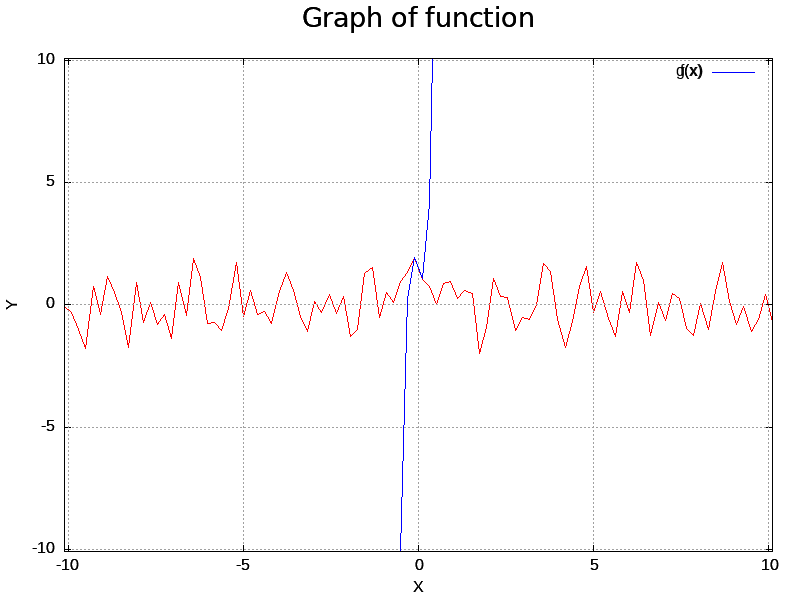
\includegraphics[width=0.8\linewidth]{Images/graphic0.png}
	\caption{\label xGraph of function.}
\end{figure}
Исходная функция: $$ \cos(5 \cdot x + 7) ^{3}  + \sin(x^{7}  + 8)  $$
Производная выражения: $$ 3 \cdot \cos(5 \cdot x + 7) ^{2}  \cdot -1 \cdot \sin(5 \cdot x + 7)  \cdot 5 + \cos(x^{7}  + 8)  \cdot 7 \cdot x^{6}  $$
Разложение в ряд Тейлора g(x) = $$ 1.41785 + -5.60116 \cdot x + 8.33705 \cdot x^{2}  + 127.92 \cdot x^{3}  $$

\addcontentsline{toc}{chapter}{bibname}
\bibliographystyle{utf8gost705u}
\bibliography{biblio}

\end{document}
